\documentclass[12pt]{article}
\usepackage[margin=1in]{geometry}
\usepackage{longtable}
\usepackage{hyperref}
\usepackage{enumitem}
\usepackage{array}
\usepackage{tikz}
\usetikzlibrary{arrows.meta, positioning, shapes.geometric}
\title{PD-Intranet: Role-Based SharePoint Resource Center}
\author{Group 10}
\date{\today}
\begin{document}
\maketitle
\tableofcontents
\newpage

\section{Software Design Document}
\section{Version History}
\begin{longtable}{|p{1in}|p{1.3in}|p{1.4in}|p{2.6in}|}\hline
Version & Snapshot & Date & Revision Notes \\ \hline
1.0 & Snapshot 1 & TBD & Initial architecture and document structure. \\ \hline
1.1 & Snapshot 2 & TBD & Added role filtering and authentication design. \\ \hline
1.2 & Snapshot 3 & TBD & Added hoteling, workload, directory, and analytics module designs. \\ \hline
1.3 & Snapshot 4 & TBD & Finalized deployment, testing, and future work notes. \\ \hline
\end{longtable}

\section{Introduction}
This Software Design Document explains how PD-Intranet is designed to meet the SRS requirements. It focuses on architecture, components, data flow, UI, security, and deployment.

\section{System Architecture}
\begin{center}
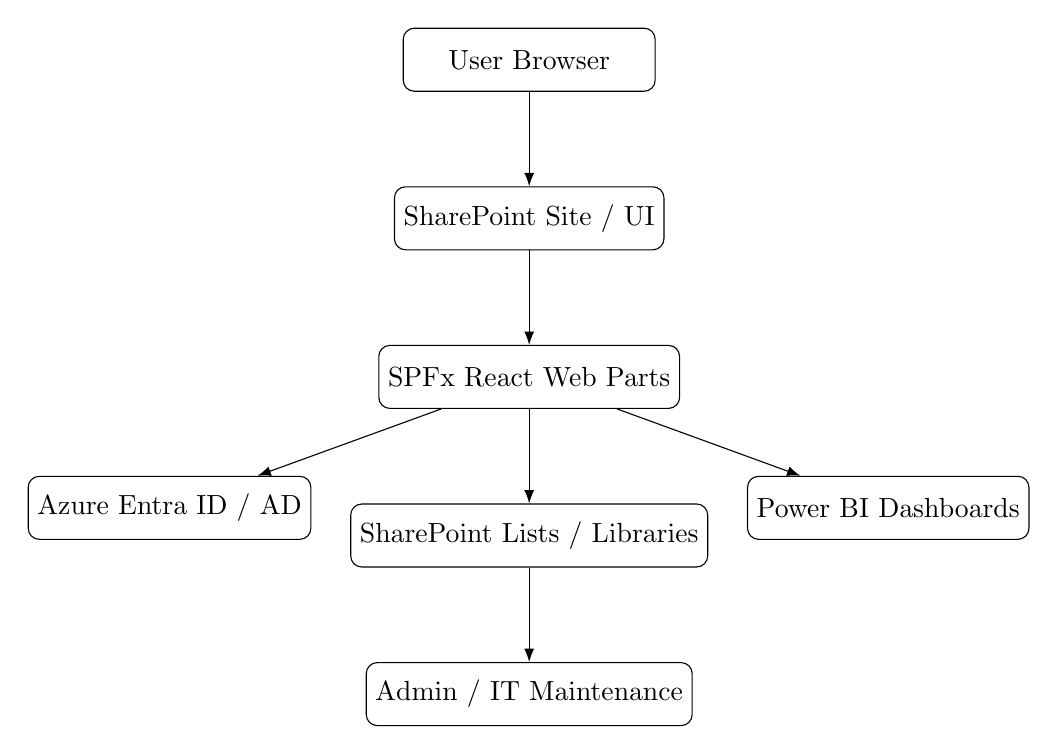
\begin{tikzpicture}[node distance=1.2cm, box/.style={rectangle, draw, rounded corners, align=center, minimum width=3.2cm, minimum height=.8cm}, arrow/.style={-Latex}]
\node[box] (user) {User Browser};
\node[box, below=of user] (sharepoint) {SharePoint Site / UI};
\node[box, below=of sharepoint] (spfx) {SPFx React Web Parts};
\node[box, below left=of spfx] (identity) {Azure Entra ID / AD};
\node[box, below=of spfx] (data) {SharePoint Lists / Libraries};
\node[box, below right=of spfx] (powerbi) {Power BI Dashboards};
\node[box, below=of data] (admin) {Admin / IT Maintenance};
\draw[arrow] (user) -- (sharepoint);
\draw[arrow] (sharepoint) -- (spfx);
\draw[arrow] (spfx) -- (identity);
\draw[arrow] (spfx) -- (data);
\draw[arrow] (spfx) -- (powerbi);
\draw[arrow] (data) -- (admin);
\end{tikzpicture}
\end{center}

\section{Component Design}
\subsection{Authentication and Role Sync}
Users sign in with Microsoft credentials. The system checks role information through Azure Entra ID or Active Directory groups.

\subsection{SPFx Frontend}
The frontend is made of reusable React components. Each web part handles one feature such as announcements, directories, workload views, or procedure checklists.

\subsection{Data Layer}
Data is stored in SharePoint lists and document libraries. PnP.js and Microsoft Graph API are used to retrieve and filter data.

\subsection{Analytics Layer}
Power BI dashboards are embedded or linked for approved roles.

\section{User Interface Design}
\begin{itemize}
\item Home Dashboard
\item Role-Based Resource Page
\item Office Hoteling Page
\item Attorney Workload Page
\item Expert Witness Directory
\item CDD Resource Guide
\item Urgency Portal
\item Staff Directory
\item Admin / Maintenance Page
\end{itemize}

\section{Security Design}
\begin{itemize}
\item Authentication is handled through Microsoft identity services.
\item Authorization is role-based.
\item Restricted pages require the correct Azure/AD role.
\item Secrets must not be committed to GitHub.
\end{itemize}

\section{Deployment Design}
The intended deployment is through SharePoint App Catalog as an SPFx package. A development Docker setup may be used for local planning and placeholder services.

\section{Future Work}
\begin{itemize}
\item Mobile-friendly improvements
\item More analytics
\item Automated onboarding/offboarding
\item Audit logging
\item Admin controls
\end{itemize}
\end{document}
